%% FOTO INVECE CHE TESTO DELLO SCHEMA
\begin{frame}{Photovoltaic Implant}
	\begin{figure}
		\centering
		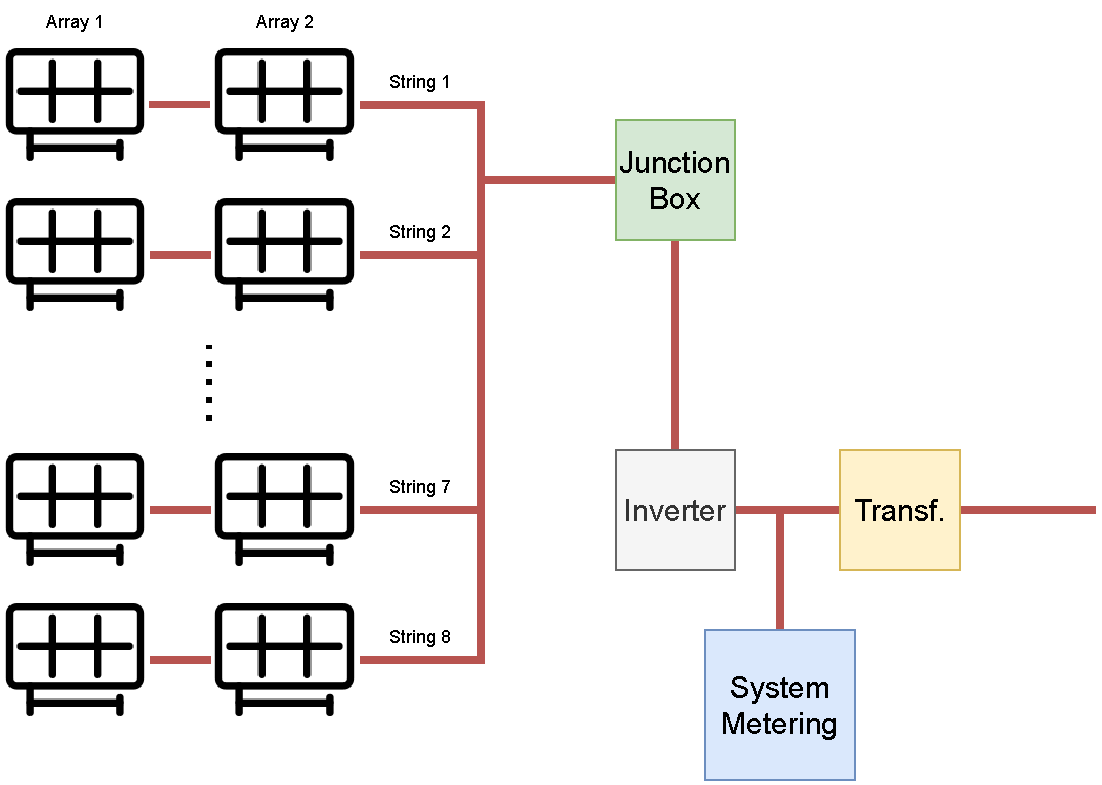
\includegraphics[width=.9\textwidth]{sections/0_intro/imgs/pvplant.pdf}
	\end{figure}
\end{frame}

%  \begin{frame}{Photovoltaic Implant}
%  \begin{columns}
%       \column[t]{.3\textwidth}
%        \begin{center}
%            \faIcon{cloud-sun}\\ 
%            \textbf{Solar Module}
%        \end{center}
%        \begin{center}
%              \footnotesize These modules consist of multiple strings of solar cells, wired in series and mounted in an aluminum frame.
%        \end{center}
%        \column[t]{.3\textwidth}
%        \begin{center}
%            \faIcon{solar-panel}\\
%            \textbf{Solar Array}
%        \end{center}
%        \begin{center}
%              \footnotesize The solar array is made up of multiple PV modules wired together in series.
%        \end{center}
%        \column[t]{.3\textwidth}
%        \begin{center}
%            \faIcon{bolt}\\
%            \textbf{Junction Box}
%        \end{center}
%        \begin{center}
%              \footnotesize The junction box serves to combine multiple series strings into one parallel circuit.
%        \end{center}
%    \end{columns}
%  \end{frame}
%  
%  \begin{frame}{Photovoltaic Implant}
%      \begin{columns}
%      \column[t]{.3\textwidth}
%      \begin{center}
%          \faIcon{sync-alt}\\
%          \textbf{Inverter}
%      \end{center}
%      \begin{center}
%              \footnotesize The inverter changes DC energy to AC energy. 
%      \end{center}
%      \column[t]{.3\textwidth}
%      %\small 
%      \begin{center}
%          \faIcon{chart-bar}\\
%          \textbf{System Metering}
%      \end{center}
%      \begin{center}
%        \footnotesize Vari strumenti che servono a misurare e determinare lo stato del sistema.
%      \end{center}
%      \column[t]{.3\textwidth}
%      \begin{center}
%          \faIcon{laptop-house}\\
%           \textbf{Load}
%      \end{center}
%      \begin{center}
%        \footnotesize Il caruco che utilizza l'energia prodotta dall'impianto. Generalmente in AC.
%      \end{center}
%  \end{columns}
%  \end{frame}